\documentclass[pdftex]{article}
\usepackage[T1]{fontenc}
\usepackage[utf8]{inputenc}
\usepackage{graphicx}
\usepackage{caption}
\usepackage{titling}

\setlength{\droptitle}{-15em}
\title{PHYS 721 Homework 4}
\author{Nick Tyler}
\date{}


\begin{document}
\maketitle
\begin{enumerate}
	\item Three Breit-Wigner curves for the decay $\phi \rightarrow K^{+} K^{- }$ are fitted to data set 1. 
		The first fit, in green, is the relatavistic Breit-wigner. The second fit, in red, is the Non-Relatavistic
		Breit-Wigner curve. \\
		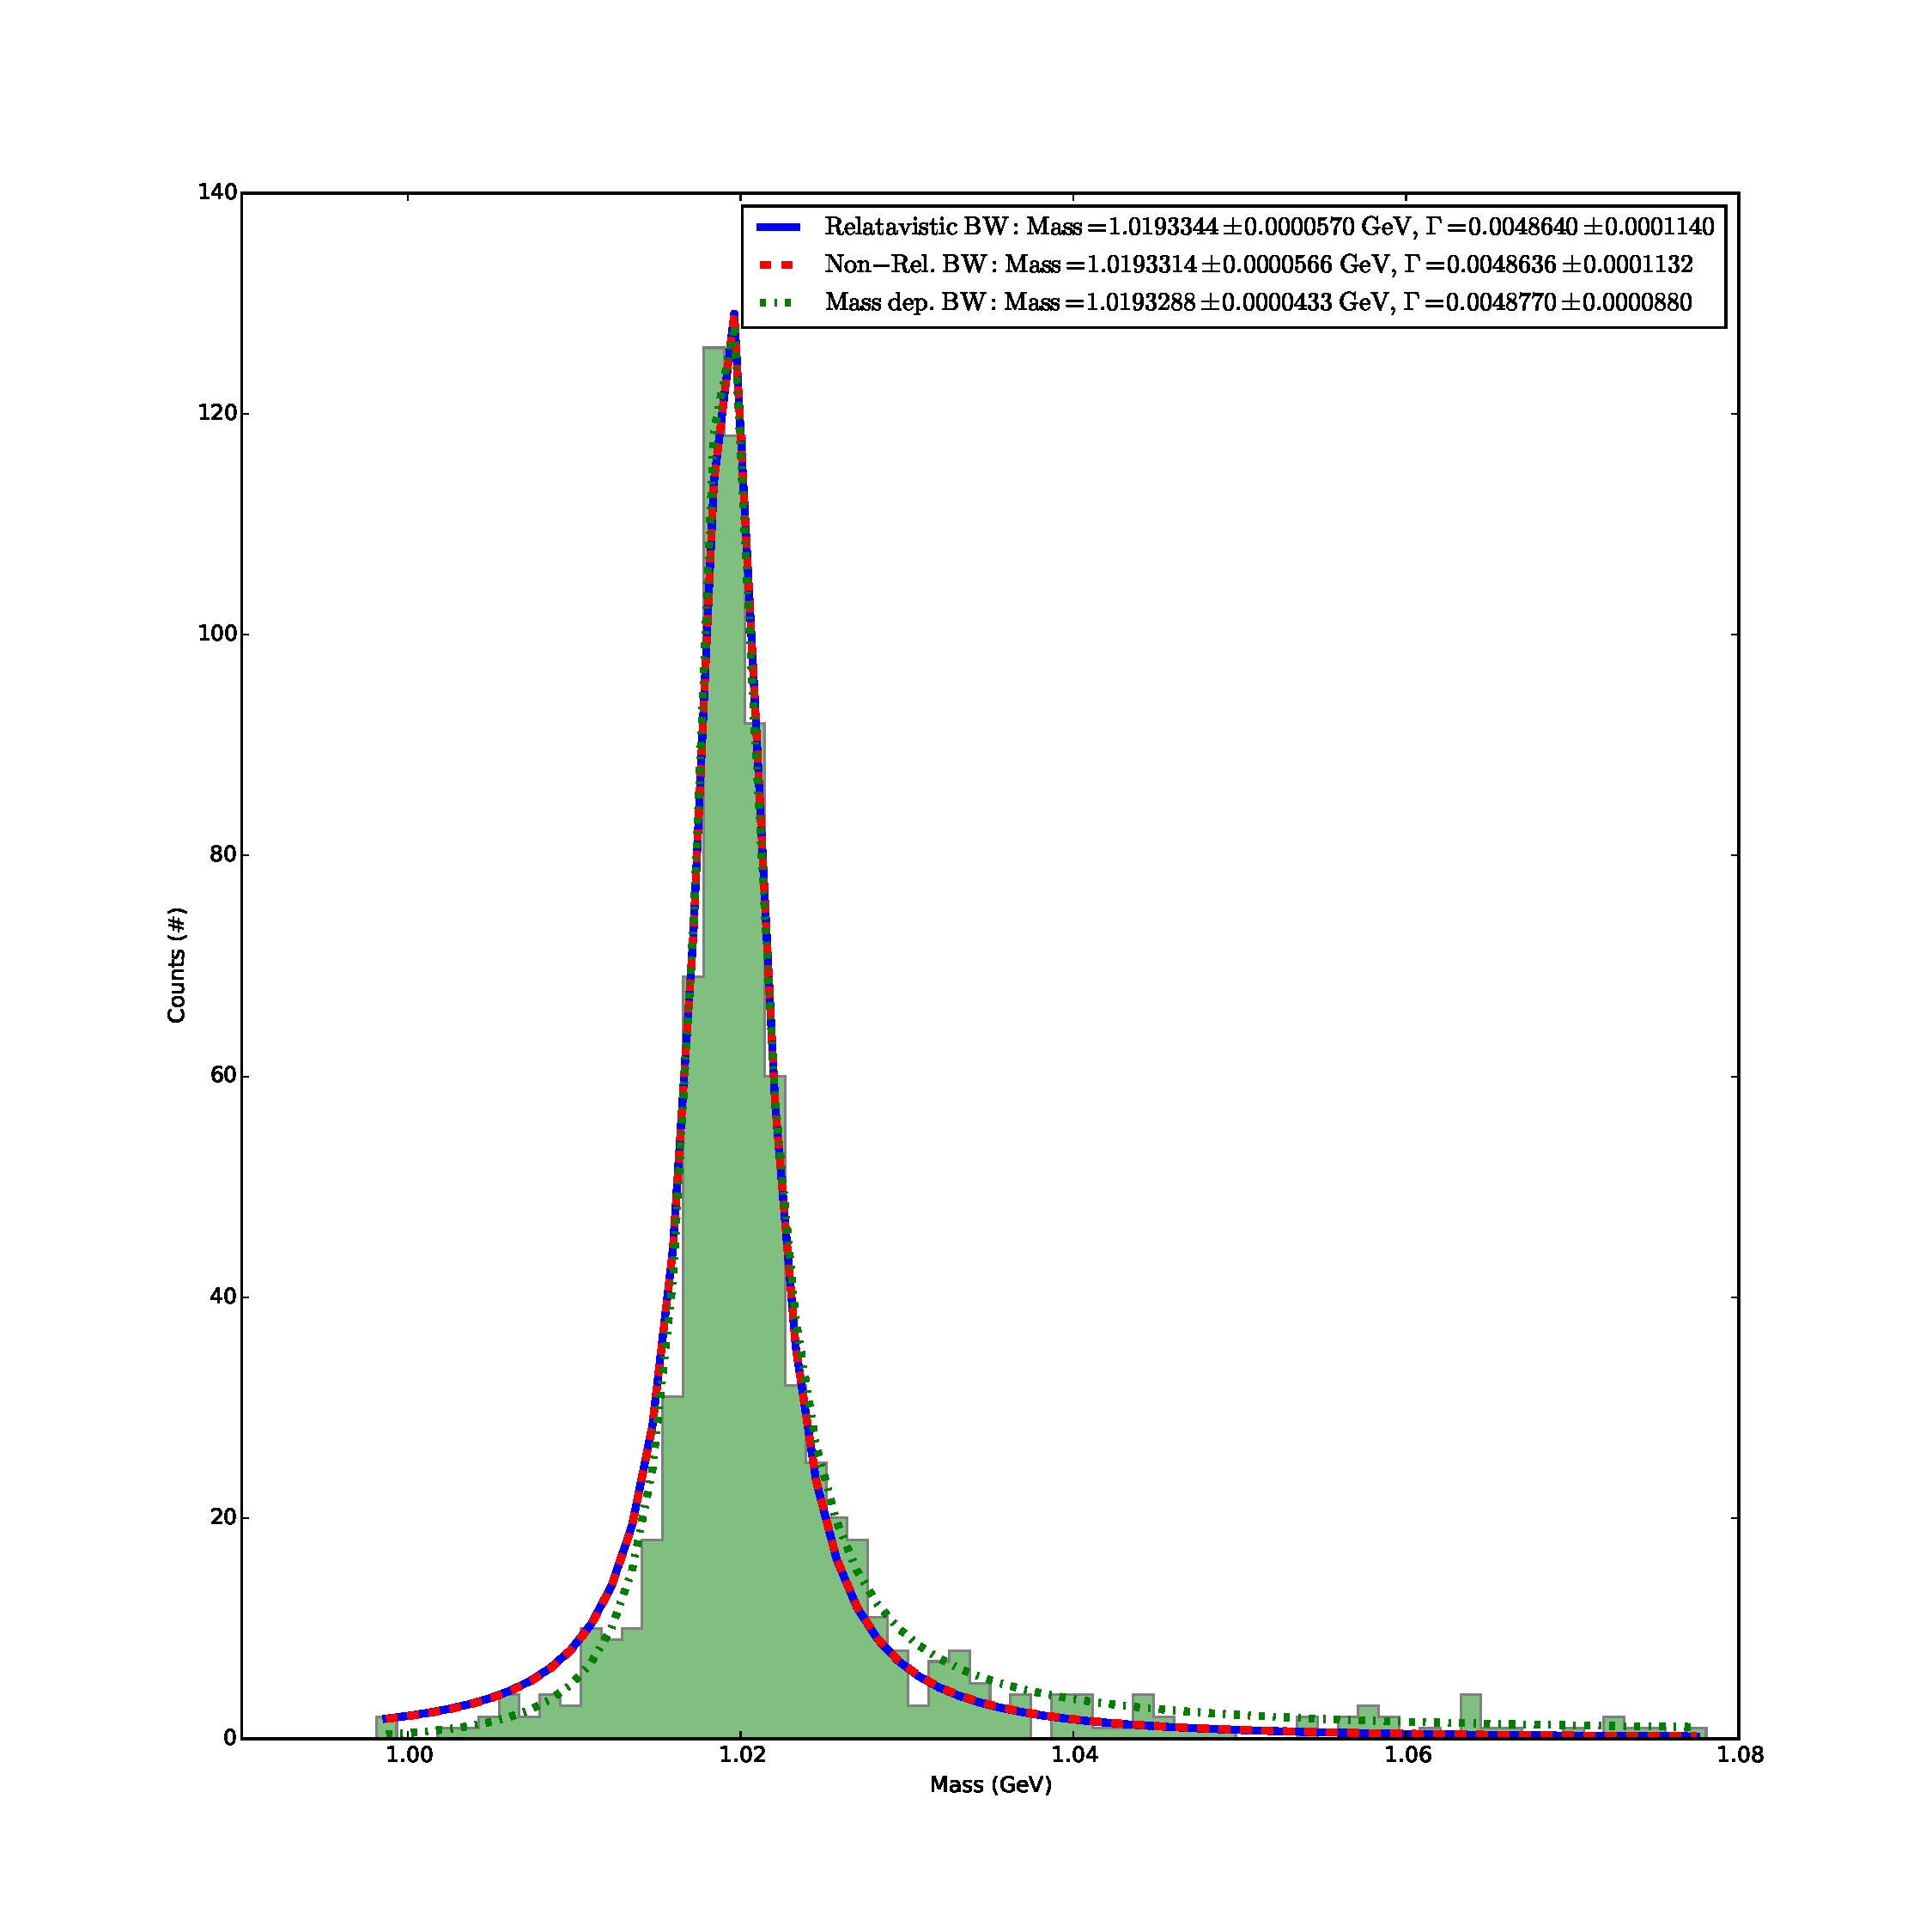
\includegraphics[scale=0.35]{Problem_1.pdf}\\
		\captionof{figure}{Three Breit-Wigner curves for, $\phi \rightarrow K^{+} K^{- }$}

	\item 
		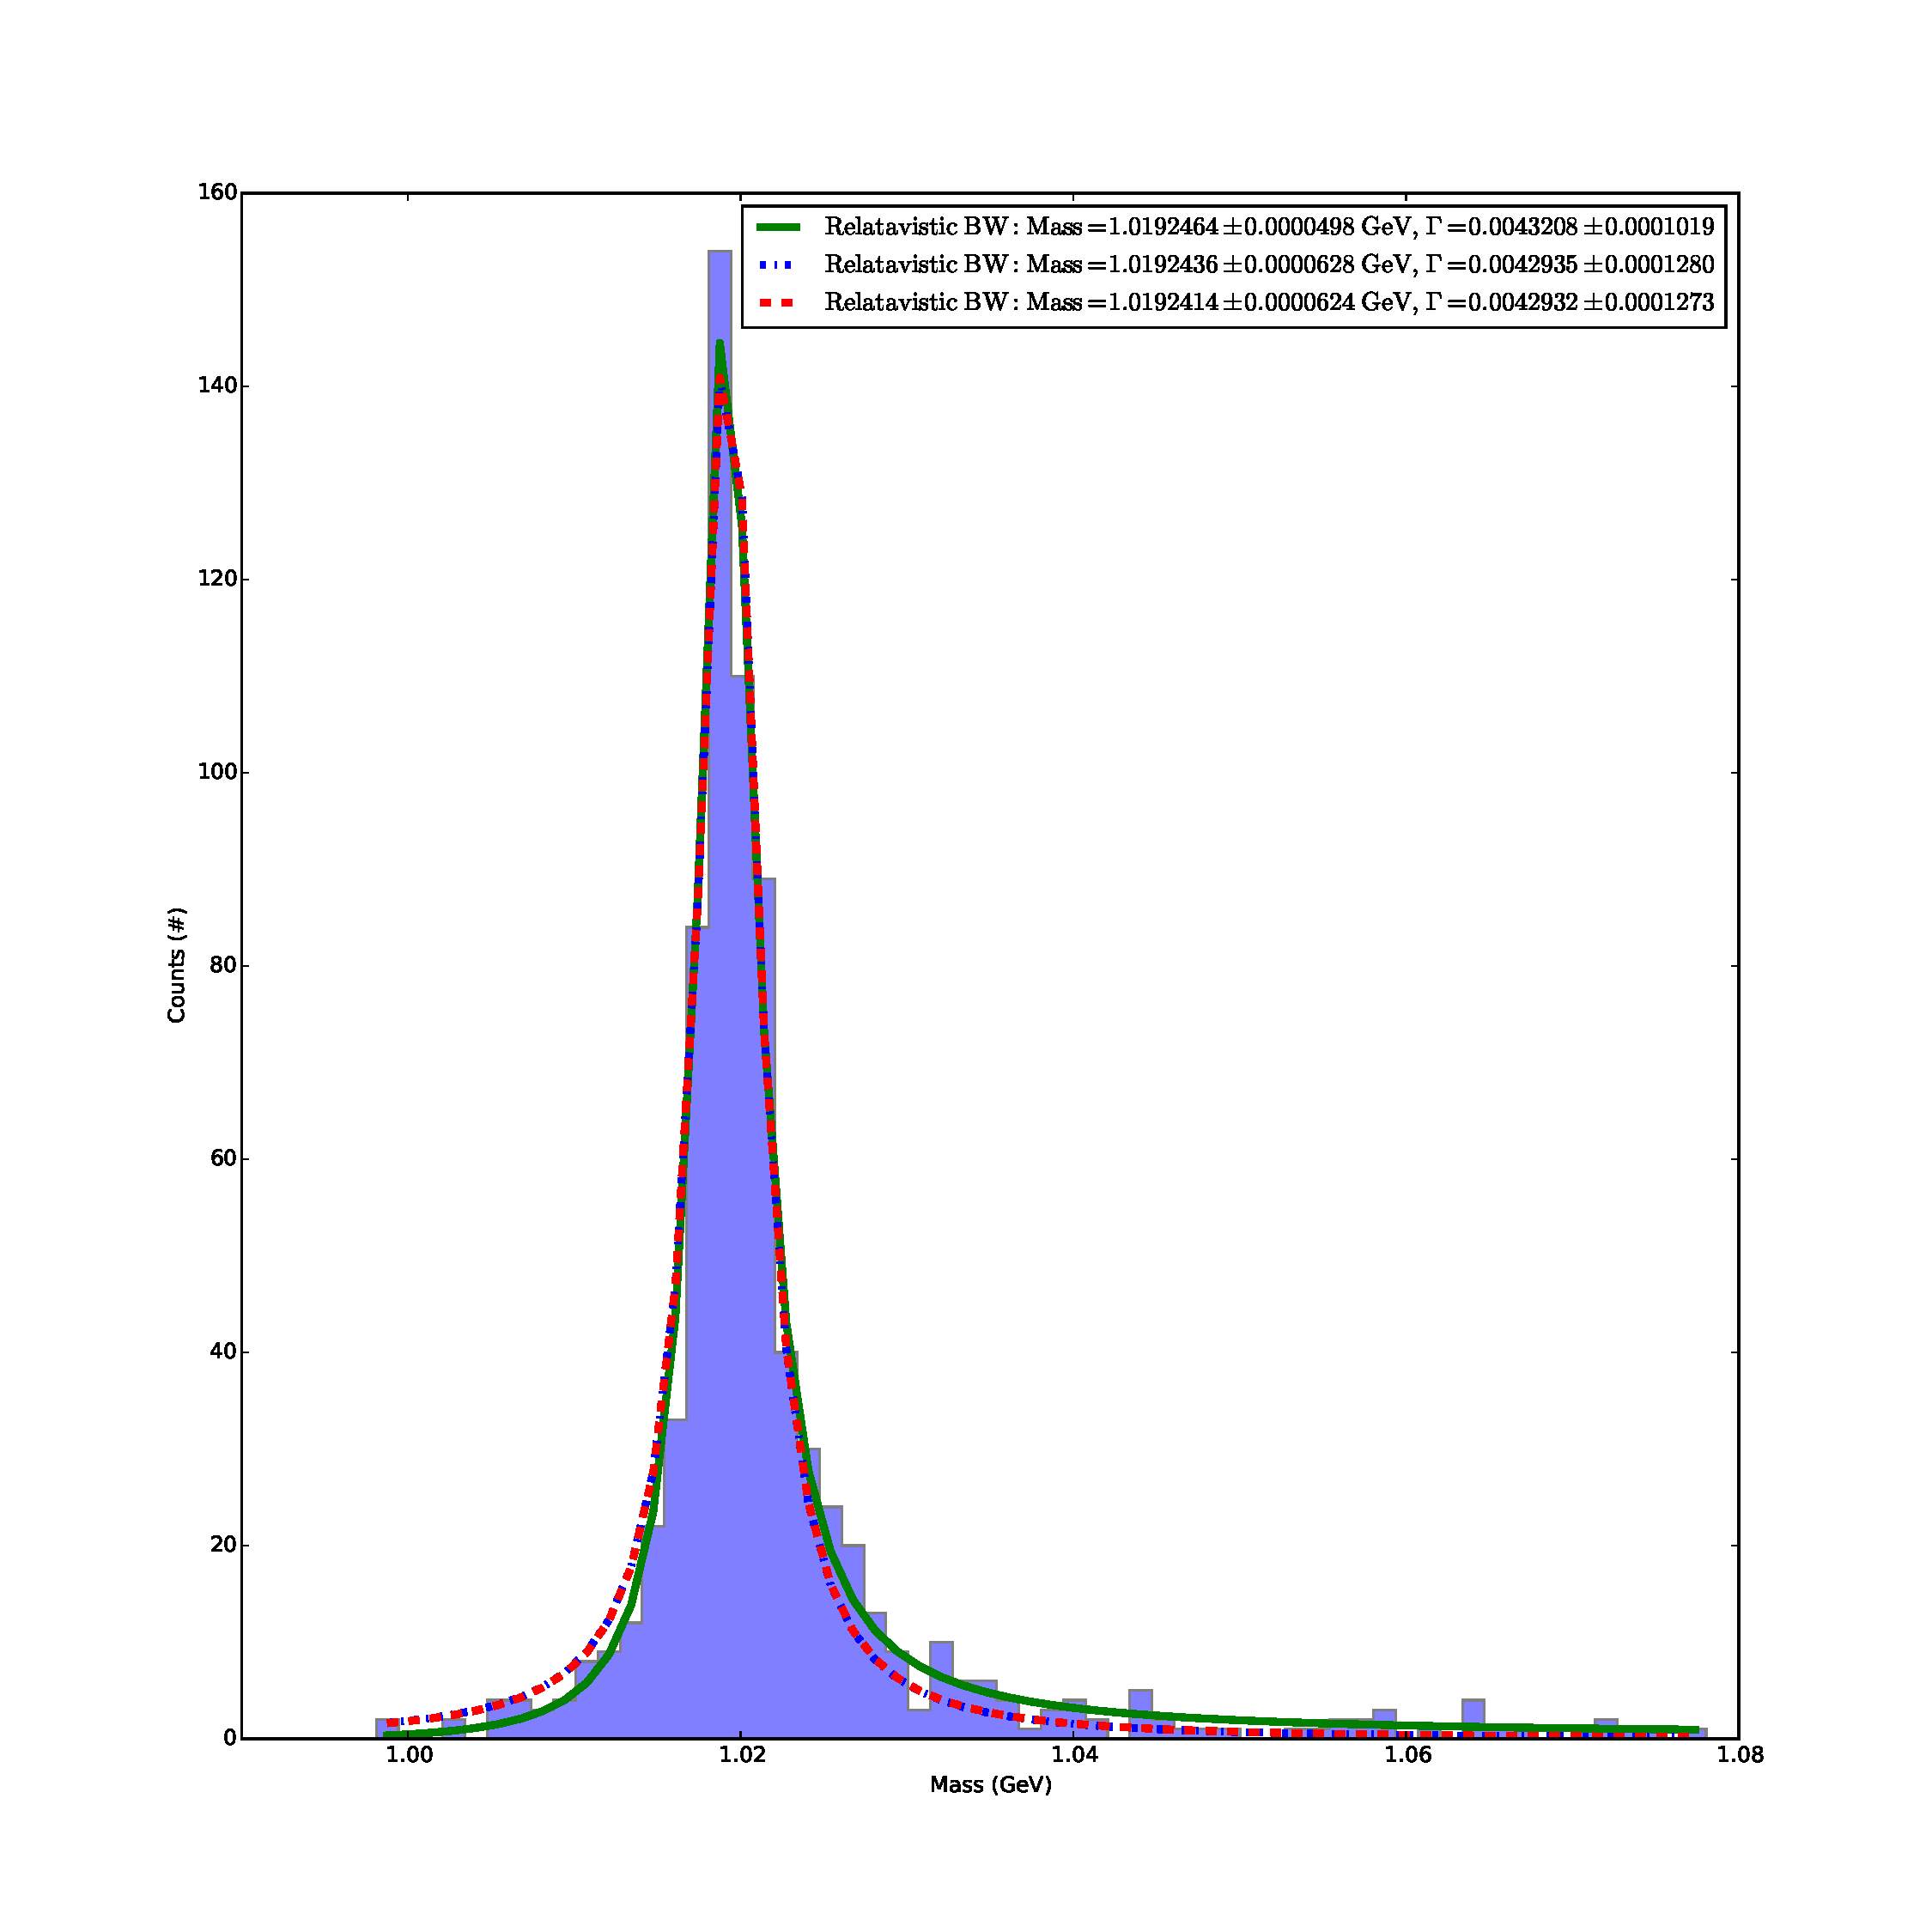
\includegraphics[scale=0.35]{Problem_3.pdf}\\
		\captionof{figure}{Three Breit-Wigner curves for, $\phi \rightarrow K^{+} K^{- }$}

\end{enumerate}

\end{document}
